% I'm trying to come up with a good format for pretty-printing my sleep data.
% This is a start; I will write most of the .tex file, and then automatically
% generate the bits that change with more data (specifically, the statitics
% and the graphs and such).

% Arun Debray, 22 June 2014

% "I haven't slept for ten days, because that would be too long." - Mitch Hedberg
% "Work 8 hours, sleep 8 hours; but not the same 8 hours" - Woody Allen
% To sleep, perchance to dream!
% If you don't go to sleep, you don't have to wake up!

\documentclass{amsart}
% Preamble for the sleep tex file.

\usepackage[margin=0.75in]{geometry}

% Graphics stuff
\usepackage{xcolor}
\definecolor{CommentColor}{HTML}{3FA5FF}
\definecolor{IDColor}{HTML}{D20DFF}
\definecolor{KeywordColor}{HTML}{0D3AFF}
\definecolor{StringColor}{HTML}{FF0D83}
\usepackage{graphicx}

% Set default font to charter and make it pretty
\usepackage{charter}
\usepackage[T1]{fontenc}
\usepackage[charter]{mathdesign}
\usepackage{microtype}

% for new commands
\usepackage{xspace}

% source code listings
\usepackage{textcomp}
\usepackage{listings}
\lstset{
	basicstyle=\scriptsize\ttfamily,
	breakatwhitespace=false,
	breaklines=true,
	commentstyle=\color{CommentColor}\textsl,
	frame=single,
%	identifierstyle=\color{IDColor},
	keywordstyle=\color{KeywordColor},
	language=Haskell,
	showstringspaces=false,
	stringstyle=\color{StringColor},
	tabsize=4,
	upquote=true
}


% TODO how fancy do I want the header to be?
\pagestyle{plain}

% Captioning and internal linking
\usepackage[
	colorlinks=true, % urlcolor and linkcolor are probably the most important
	linkcolor=IDColor,
	citecolor=CommentColor,
	filecolor=KeywordColor,
	urlcolor=StringColor
	]{hyperref}
\usepackage[all]{hypcap}

\newcommand{\readTODO}[1]{\textbf{TODO}}
\newcommand{\readStat}[1]{\textbf{\input{statistics/#1.txt}}\!\!\xspace}

\begin{document}
\title{Summary of My Sleep Data}
\author{Arun Debray\\\today}
\maketitle

\begin{quote}\textit{
``I want to default on my sleep debt!''
}\end{quote}

\begin{abstract}
Since mid-June 2014, I have kept track of when I have gone to sleep, when I have woken up, and when I napped. This data is useful, interesting, and sometimes sadly amusing. I've prepared some basic statistics on the data, as well as some notes on how I made everything work.

This document, the data, and the programs I used to generate them can be found at \url{http://stanford.edu/~adebray/Haskell/sleep/}. Any questions, comments, or concerns may be directed to me, at \href{mailto:adebray@stanford.edu}{\texttt{adebray@stanford.edu}}.
\end{abstract}

\section{Basic Statistics}
During this project, I have recorded my sleep for \readStat{numDays} days, during which I slept a grand total of \readStat{totalHours} hours. Somehow it didn't feel like quite that much.

% Look at Figure~\ref{} for a graph of how much sleep I got per night.
See Figure~\ref{raw_data} for when I went to sleep and woke up each night.
\begin{figure}[h!]
	\centering
	\label{raw_data}
	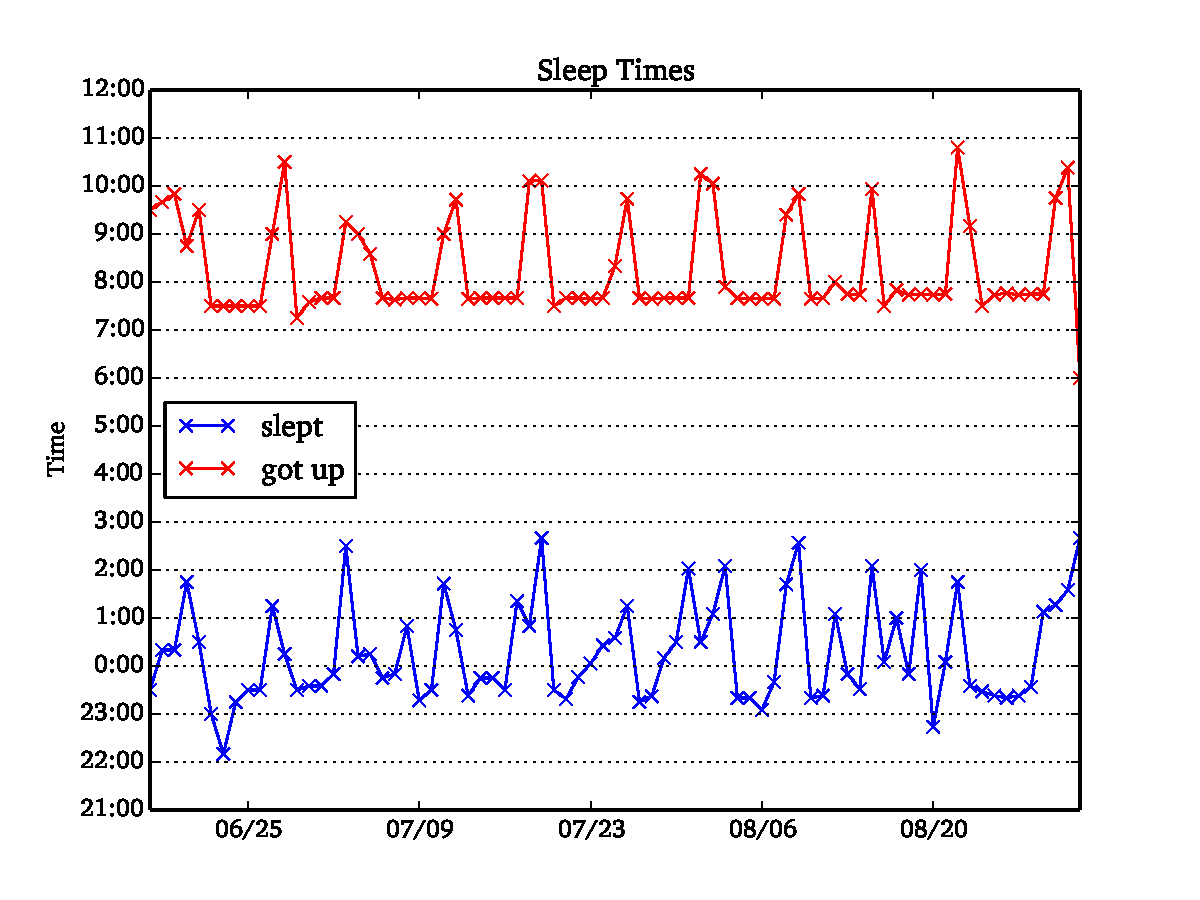
\includegraphics[width=5.5in]{plots/raw_times}
	\caption{The most basic plot: when I went to sleep and when I woke up each day.}
\end{figure}

\section{Averages}
On average, I have gotten \readStat{overallAverage} hours of sleep per night. If naps are excluded, this is reduced to \readStat{overallNoNaps} hours per night.

The average has, of course, changed over time. In the last seven days, I've averaged \readStat{lastWeek} hours (\readStat{weekNoNaps} without naps) and in the last 30 days, I've averaged \readStat{lastMonth} hours (\readStat{monthNoNaps} without naps). % Eventually, I will update this with yearly data.

% Check out Figures~\ref{} and \ref{} for graphs 7- and 30-day moving averages, respectively.

\section{Standard Deviations}
The standard deviation of my sleep has been \readStat{overallStdDev} hours with naps and \readStat{stdDevNoNaps} hours without them. In the last seven days, the standard deviation was \readStat{weekSD} hours (\readStat{weekSDNoNaps} hours without naps), and in the last 30 days, it was \readStat{monthSD} hours (\readStat{monthSDNoNaps} hours without naps).

\section{Per Day of the Week}
In this section, I will analyze my sleep per day of the week (averages, standard deviations, etc). However, I have yet to do that\dots{} it's a work in progress. I do have graphs of waking and sleeping times in Figures~\ref{asleep_weekly} and \ref{awake_weekly}, though.

\begin{figure}[h!]
\centering
\label{asleep_weekly}
\includegraphics[width=6.5in]{plots/asleep_box}
\caption{Box plots for when I went to sleep, broken down per day of the week. The boxes represent quartiles, so that each box contains $75\%$ of the data of that day, and the whiskers contain the remaining $25\%$; the bar across the box represents the mean. Outlier values are represented by the diamonds.}
\end{figure}
\begin{figure}[h!]
\centering
\label{awake_weekly}
\includegraphics[width=6.5in]{plots/awake_box}
\caption{Much the same as Figure~\ref{asleep_weekly}, this is a box plot of when I woke up over days of the week, with diamonds as outliers.}
\end{figure}

\section{Per Hour of the Day}
Here I attempt to answer the question: how likely am I to be asleep at a given hour? % add total, last seven days, and last 30 days answers to the question.
See Figure~\ref{probs} for the answer over the entire data collection period. A probability $p$ means that on an arbitrary day, I am asleep at that time with probability $p$.
\begin{figure}[h!]
	\centering
	\label{probs}
	\includegraphics[width=5.5in]{plots/sleep_probs}
	\caption{A plot of time versus how probable it is that I am asleep at a given time.}
\end{figure}

\section{Some Source Code}
\lstinputlisting[caption=Common notions for programs.]{SleepTime.hs}
\lstinputlisting[caption=Used to record data.]{enter_data.hs}
\lstinputlisting[caption=Used to generate statistics.]{writeStatistics.hs}
\lstinputlisting[language=Python, caption=Used to make plots.]{plotMaker.py}
\end{document}
